\section{C语言简介}


\begin{frame}\ft{C的起源}
\begin{itemize}
    \item 
      \red{产生时间:}1972-1973年\\[0.2in]
    \item 
      \red{产生地点:}美国贝尔实验室\\[0.2in]
    \item 
      \red{创始人:}Dennis Ritchie \& Ken Thompson\\[0.2in]
    \item  
      \red{目的:}改写Unix系统\\[0.2in]
    \item 
      \red{荣誉:}美国国家技术奖章(1999)
    \end{itemize}
\end{frame}



\begin{frame}\ft{C的起源}
\begin{figure}
\centering
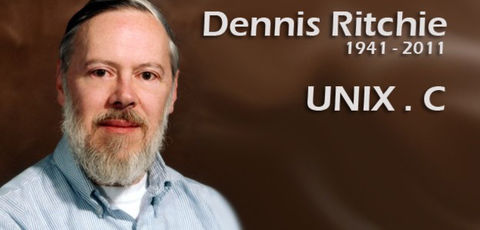
\includegraphics[width=4in]{ch01/fig/Ritche}
\end{figure}
\end{frame}

\begin{frame}\ft{C的起源}
\begin{figure}
\centering
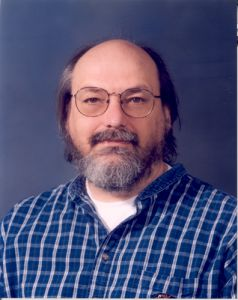
\includegraphics[width=2in]{ch01/fig/Thompson}
\caption{Ken Thompson (1942-)}
\end{figure}
\end{frame}

\begin{frame}\ft{C的起源}
\begin{figure}
\centering
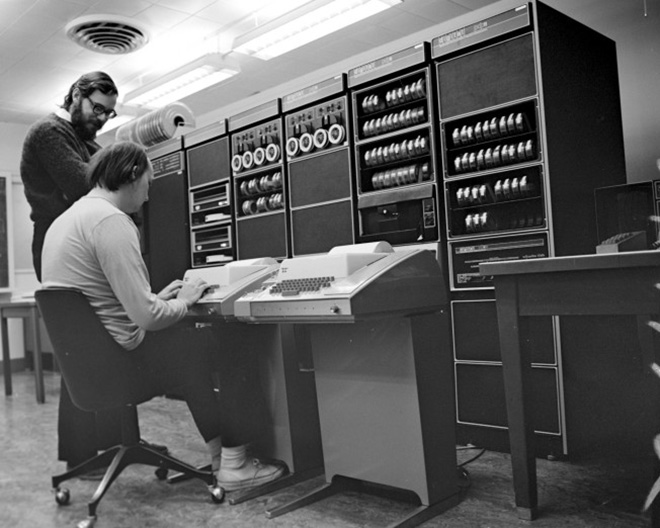
\includegraphics[width=3in]{ch01/fig/Ritche_Thompson}
\caption{Dennis Ritchie和Ken Thompson(1972年)}
\end{figure}
\end{frame}

\begin{frame}\ft{C的起源}
1983年,Dennis Ritchie和Ken Thompson一起获得了图灵奖,理由是:“研究发展了通用的操作系统理论,尤其是实现了Unix操作系统”。
\end{frame}

\begin{frame}\ft{关于Ritche的评价}
\begin{figure}
\centering
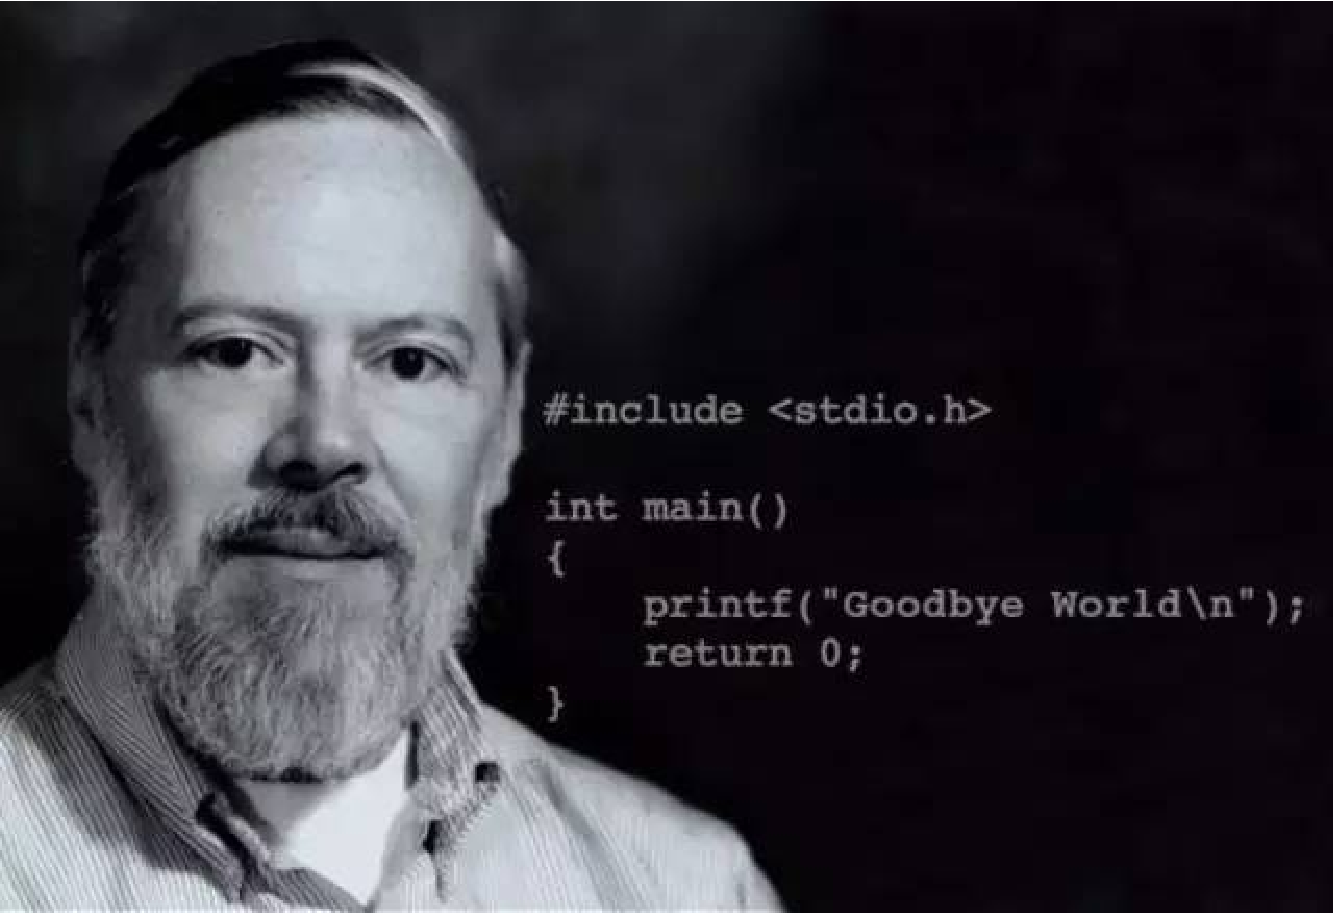
\includegraphics[width=3.5in]{ch01/fig/Ritche1}
\end{figure}

\end{frame}

\begin{frame}\ft{关于Ritche的评价1}

“当乔布斯去世时,享受到了声势浩大的追思。相形之下,里奇先生对当代科技进程做出了更大的贡献,可公众甚至不知道他是谁,这十分不公平。” 
\end{frame}

\begin{frame}\ft{关于Ritche的评价2}
“如果说,乔布斯是可视化产品中的国王,那么里奇就是不可见王国中的君主。乔布斯的贡献在于,他如此了解用户的需求和渴求,以至于创造出了让当代人乐不思蜀的科技产品。然而,却是里奇先生为这些产品提供了最核心的部件,人们看不到这些部件,却每天都在使用着。”
\end{frame}

\begin{frame}\ft{关于Ritche的评价3}
\red{“牛顿说他是站在巨人的肩膀上,如今,我们都站在里奇的肩膀上。”}

\end{frame}


\begin{frame}\ft{C的地位}
\begin{itemize}
\item  C拥有汇编语言的力量和便利性,其运行方式更接近于硬件系统;\vskip.1in
\item  C所提供的数据结构,力发千钧,足以贯穿所有高层和底层的语言;
\end{itemize}

\end{frame}

\begin{frame}\ft{C的地位}
\begin{itemize}
\item
C的开发是科技史上不可磨灭的伟大贡献,因为这个语言把握住了计算机科技中一个至关重要的并且是恰到好处的中间点,一方面它具备搭建高层产品的能力,另一方面又能够对于底层数据进行有效控制。正是由于这种关联性和枢纽性作用,决定了 C所导向的近三十年来计算机编程主流方式。
\end{itemize}

\end{frame}

\begin{frame}\ft{C的优点}
\begin{itemize}
\item[(1)] \red{设计特性}\quad 融合了控制特性,使得用户可以采用自顶而下的结构化编程,以及模块化的设计,从而使编写出的程序更可靠、更易懂 \\[0.1in] 
 
\item[(2)] \red{高效性}\quad  代码紧凑且运行速度快,可以表现出只有汇编语言才具有的精细控制能力  \\[0.1in] 
 
\item[(3)] \red{可移植性}\quad 在一个系统上编写的程序经过很少改动或不经修改就可以在其他系统上运行 \\[0.1in] 
 
\item[(4)] \red{强大的功能与灵活性}\\[0.1in] 
\begin{itemize}
\item  强大而灵活的UNIX操作系统便是用C编写的   \\[0.1in] 
\item  其他语言(如Fortran、Python等)的许多编译器和解释器都是用C编写的\\[0.1in] 
\end{itemize}

\item[(5)] \red{面向程序员}\\[0.1in] 
\begin{itemize}
\item 允许你访问硬件,并可以操纵内存中的特定位  \\[0.1in] 
\item 具有丰富的运算符供选择,让你能够简洁地表达自己的意图 
\end{itemize}
\end{itemize}

\end{frame}

\begin{frame}\ft{C的缺点}
\begin{itemize}
\item[(1)]  在表达方面的自由会增加风险。\\[0.1in]
\item[(2)]  对指针的使用,可能导致你会犯难以追踪的编程错误。\\[0.1in]
\item[] \red{自由的代价是永远的警惕。}\\[0.2in]
\item[(3)]  其简洁性与丰富的运算符相结合,可能会产生极难理解的代码。\\[0.1in]
\item[]  \red{含糊代码竞赛}
\url{www.ioccc.org}
\end{itemize}
\end{frame}
